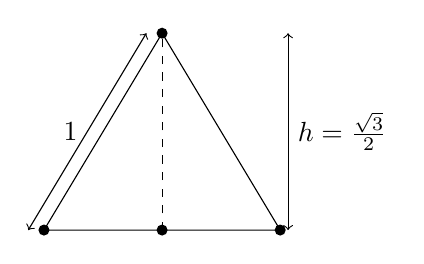
\begin{tikzpicture}

\coordinate (A) at (-2, 0);
% \node at (A) [below]{$A$};
\fill (A)  circle[radius=2pt];

\coordinate (B) at (1,0);
% \node at (B) [below]{$B$};
\fill (B)  circle[radius=2pt];

\coordinate (C) at (-0.5,2.5);
% \node at (C) [above]{$C$};
\fill (C)  circle[radius=2pt];

\coordinate (D) at (-0.5,0);
% \node at (D) [above]{$D$};
\fill (D)  circle[radius=2pt];


\draw (A) -- (B) -- (C) -- (A); 
\draw [<->] (-2.2,0) -- (-0.7,2.5) node[midway, left]{$1$};
\draw [dashed] (D) -- (C);
\draw [<->] (1.1,0) -- (1.1,2.5) node[midway, right]{$h=\frac{\sqrt{3}}{2}$};


\end{tikzpicture}